% !TEX root = slides.tex

\section{Identification}

\againframe{overview}

\begin{frame}
    \frametitle{Data Collection}

    \begin{columns}
        \begin{column}{0.6\textwidth}
            \only<1>{
                \begin{figure}
                    \centering
                    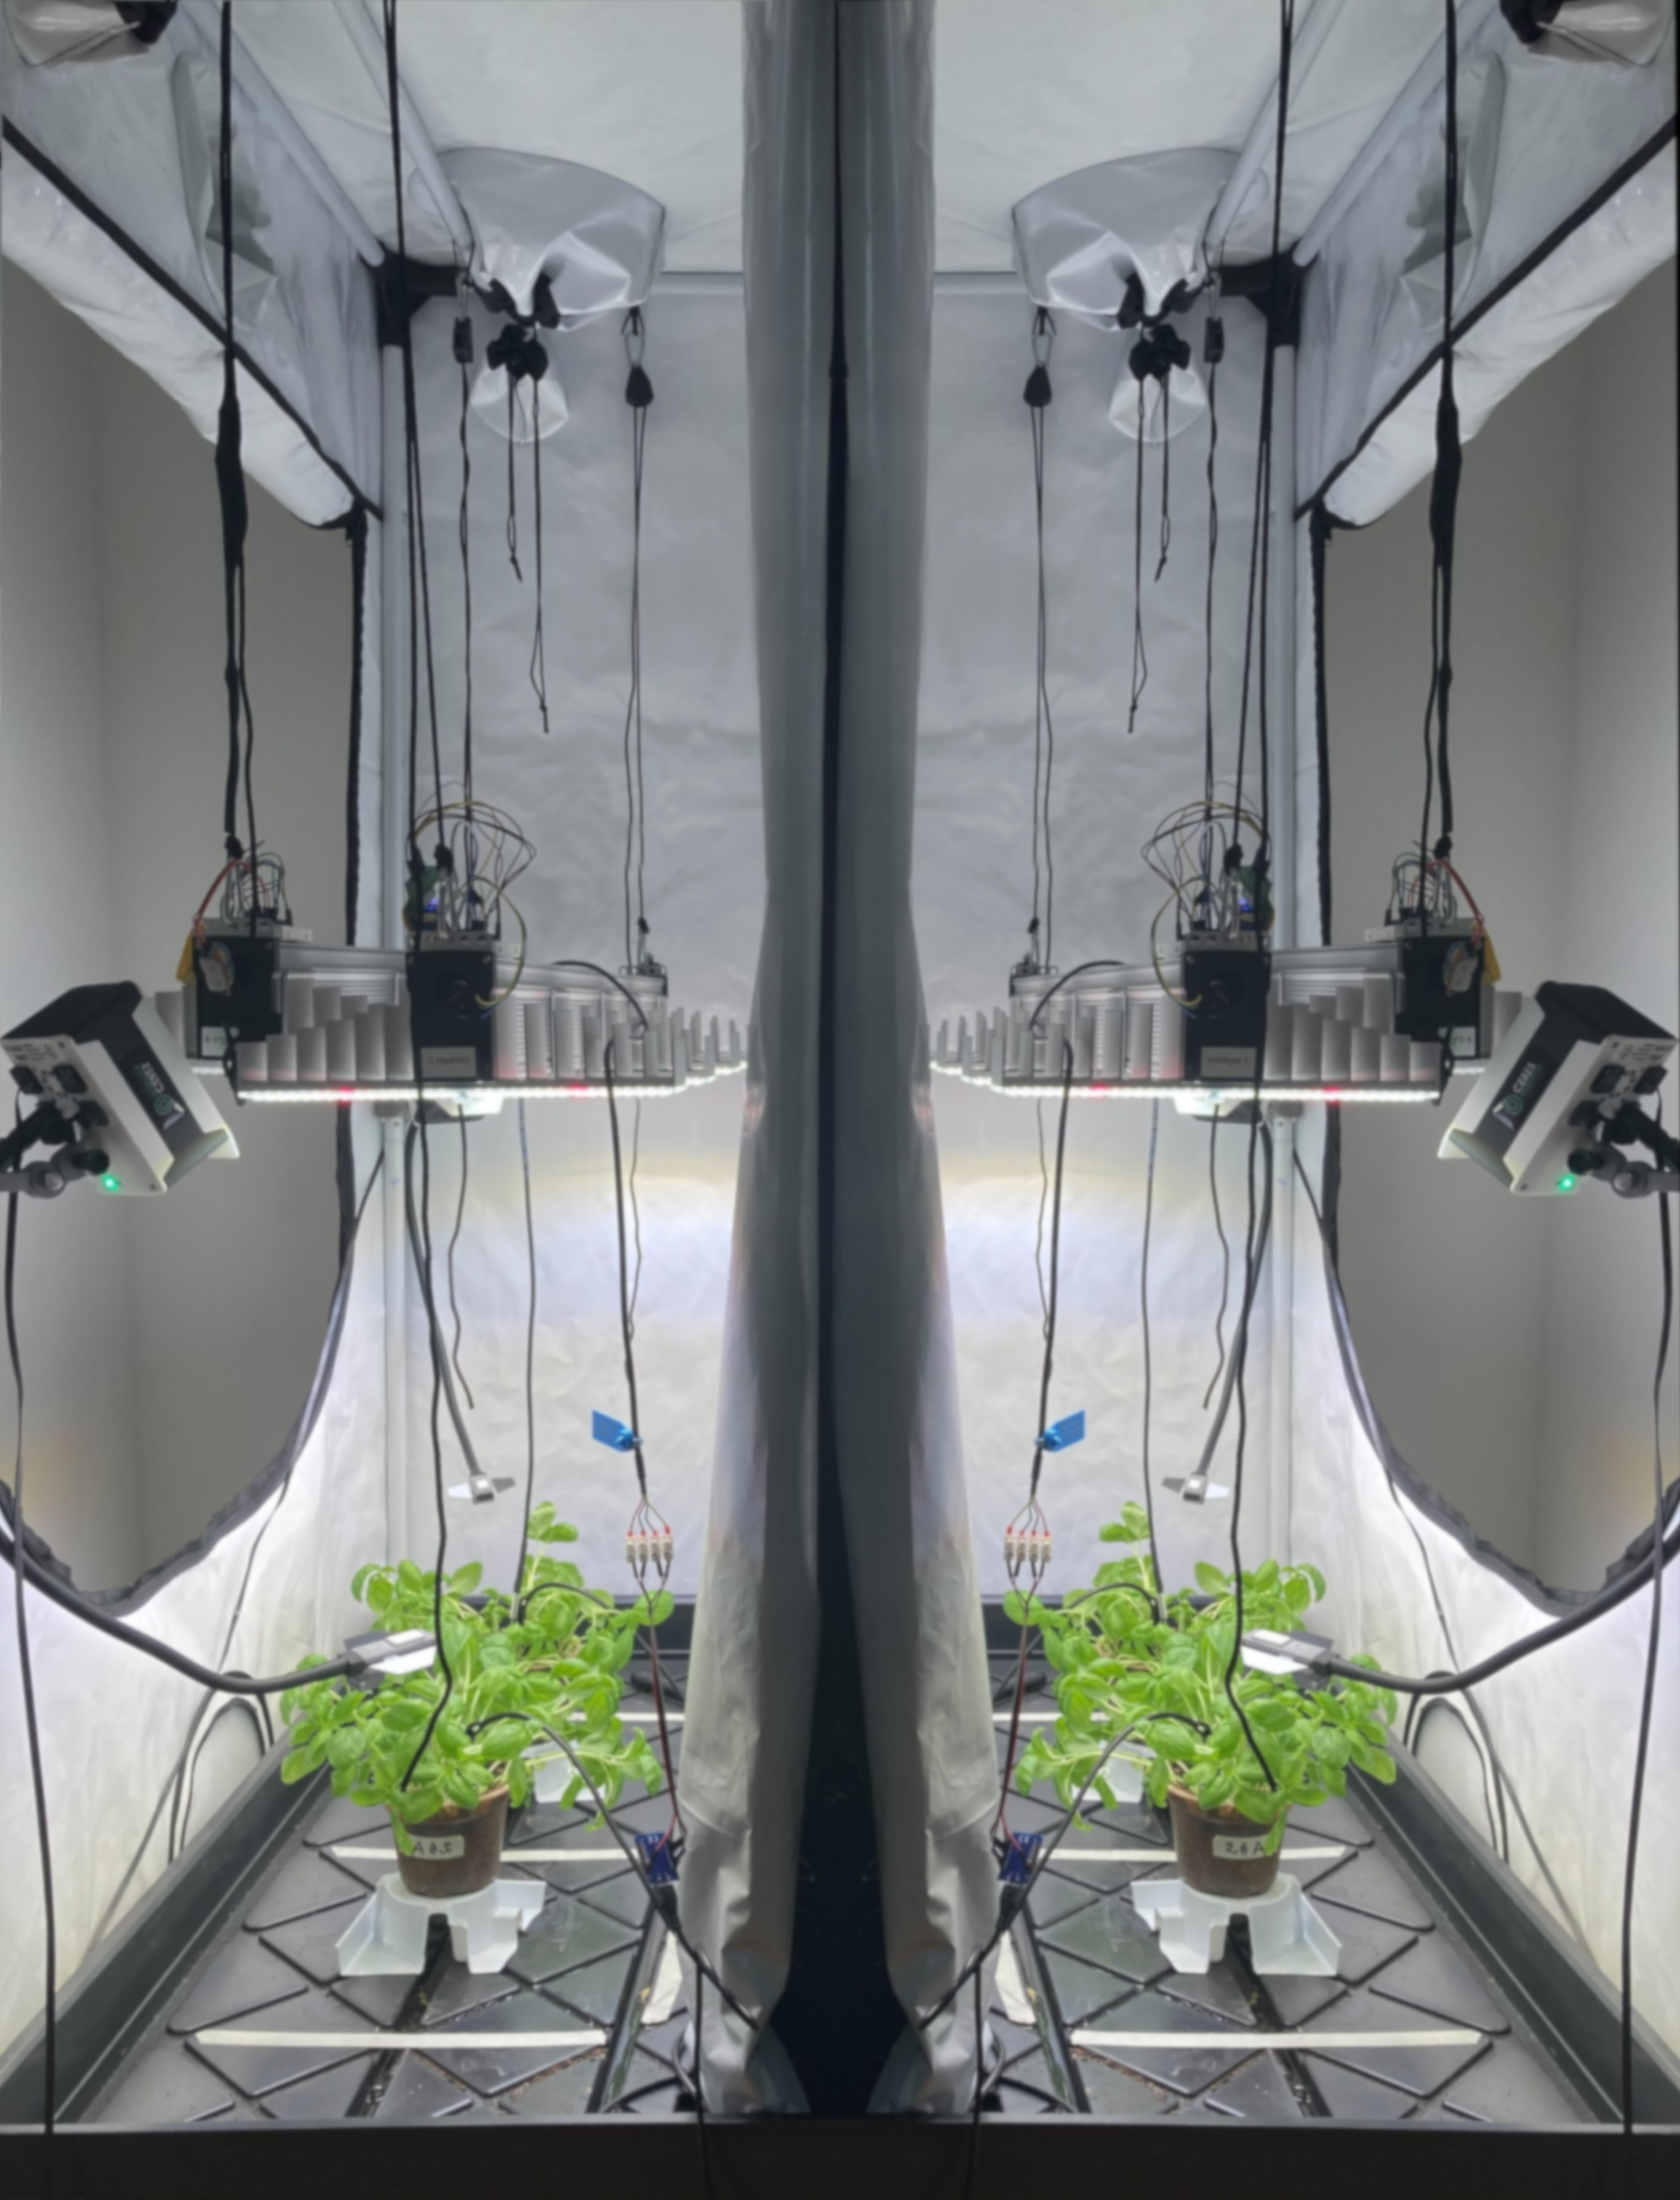
\includegraphics[scale=0.033]{figures/tent.jpg}
                    \caption{Indoor agriculture facility.}
                \end{figure}
            }
            \only<2>{
                \begin{figure}
                    \centering
                    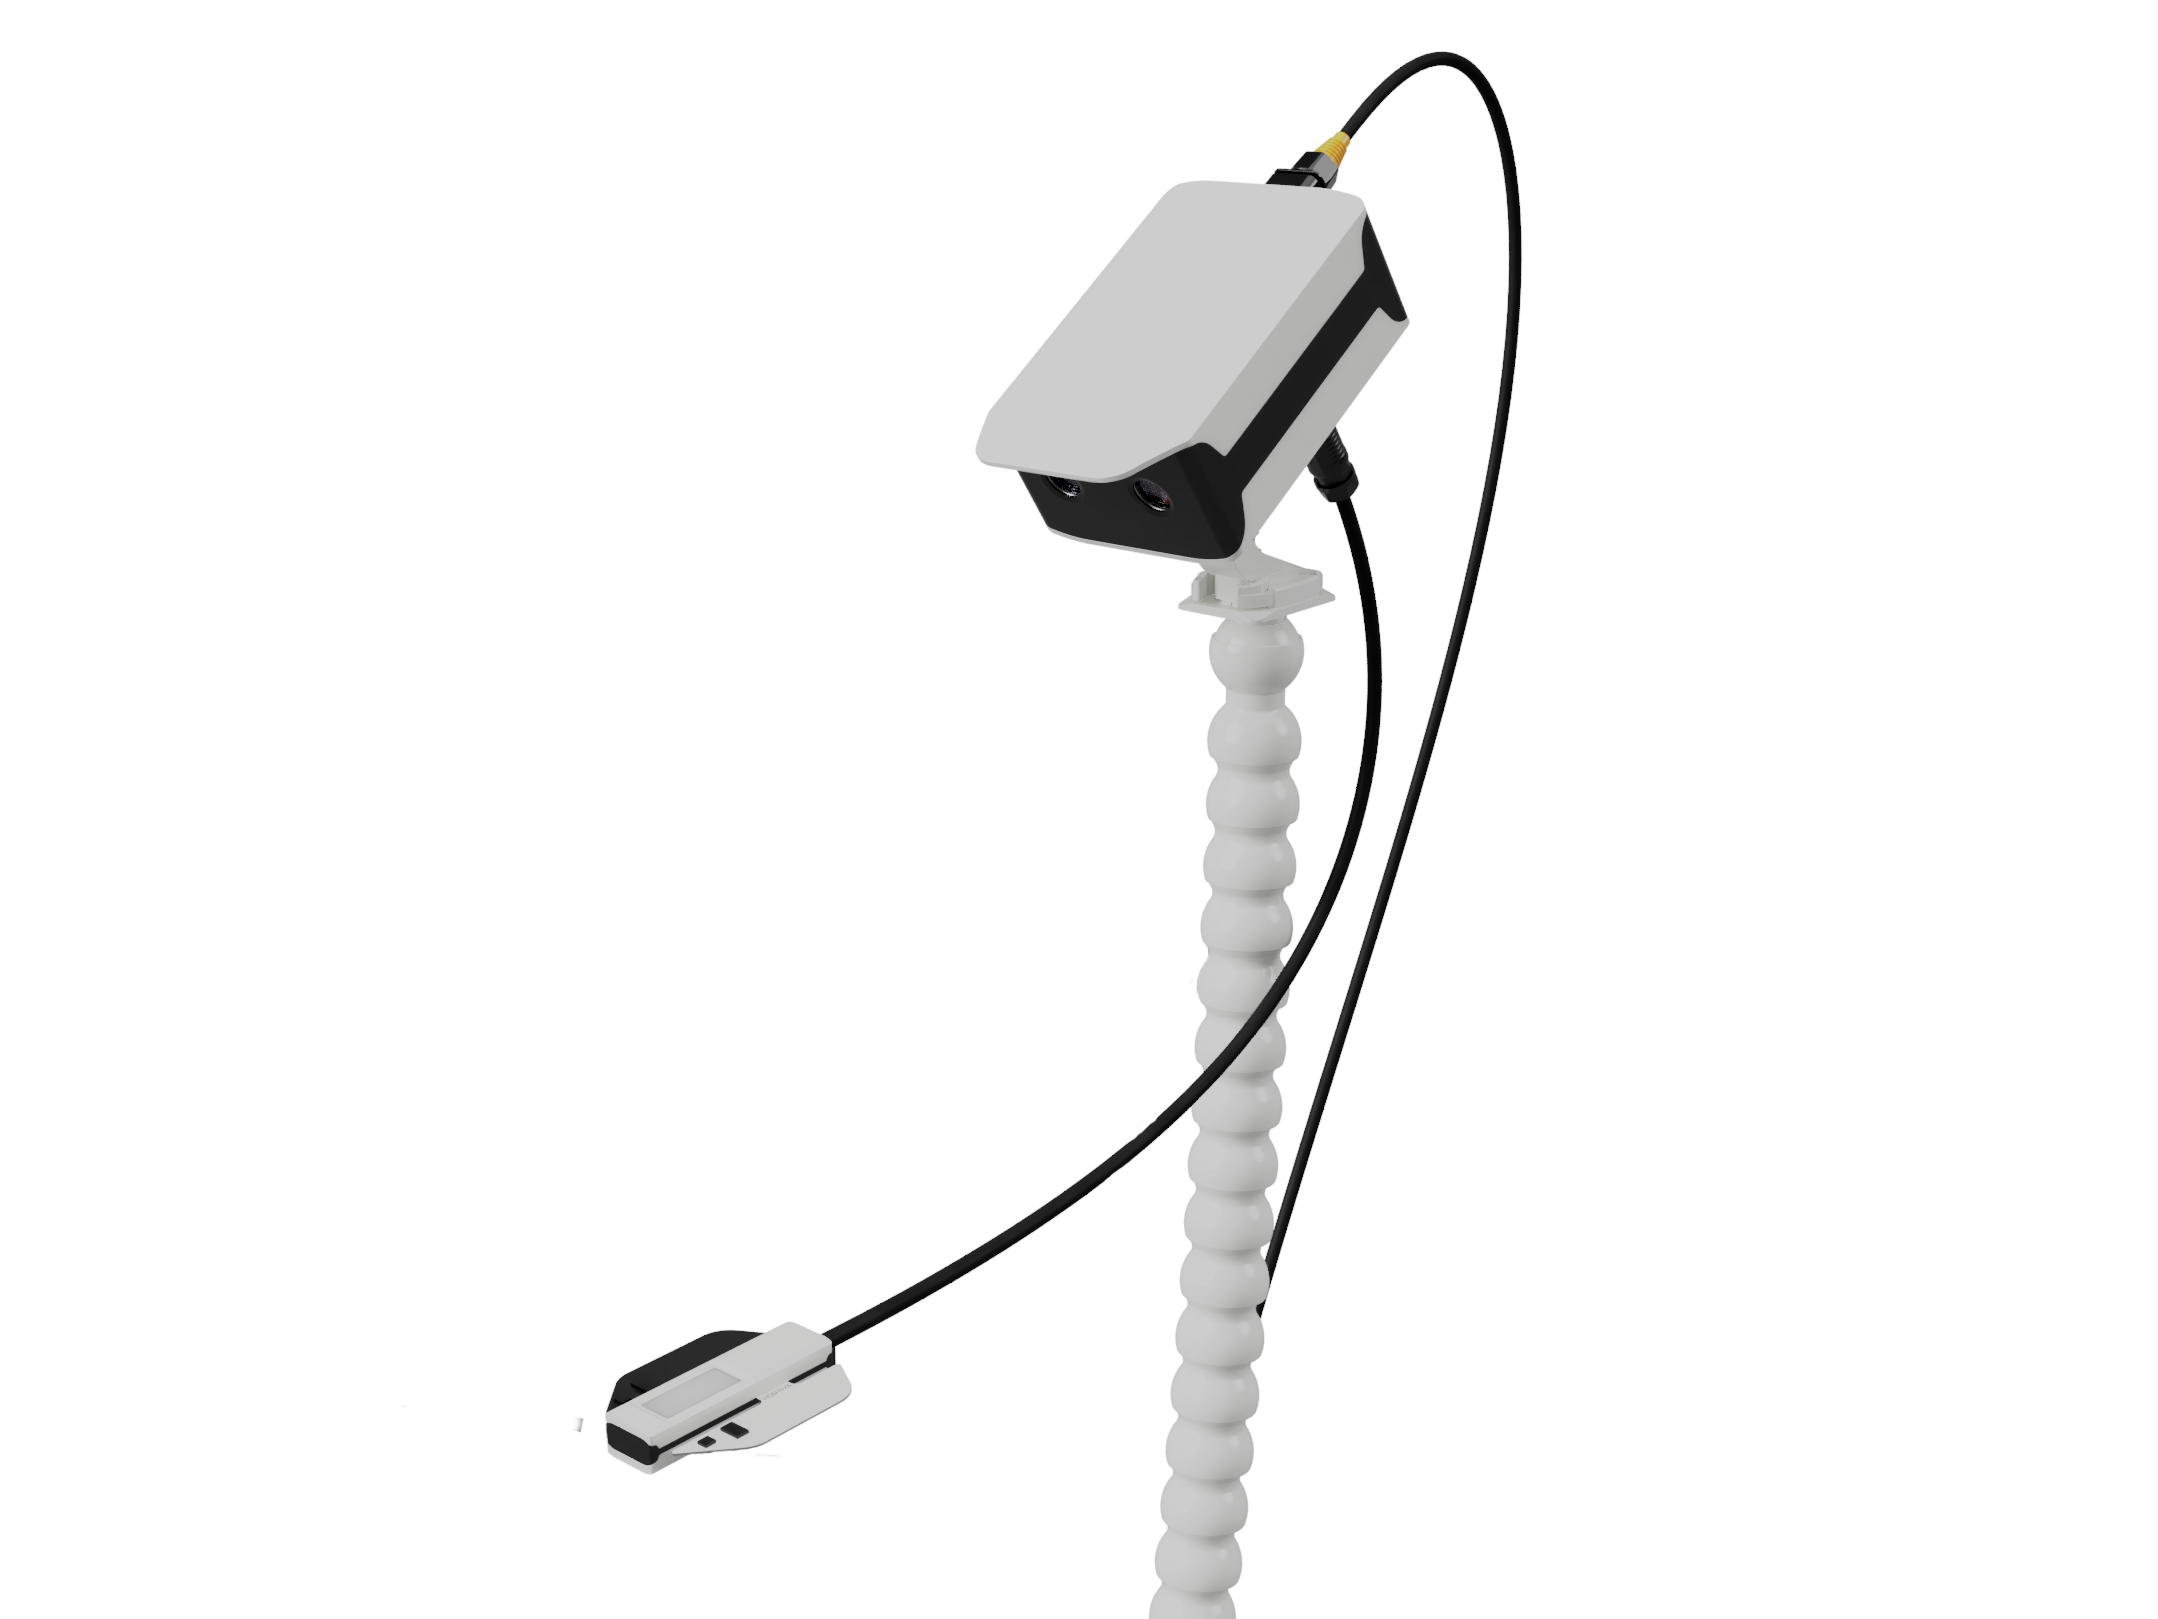
\includegraphics[scale=0.066]{figures/ceres.png}
                    \caption{Hortiya sensor system.}
                \end{figure}
            }
        \end{column}
        \begin{column}{0.4\textwidth}
            \begin{itemize}
                \item test 1 
                \item test 2
            \end{itemize}
        \end{column}
    \end{columns}
\end{frame}

\begin{frame}
    \frametitle{Plant Physiology}

    \begin{columns}
        \begin{column}{0.4\textwidth}
            \begin{itemize}
                \item test 1
                \item test 2
            \end{itemize}
        \end{column}
        \begin{column}{0.6\textwidth}
            \begin{center}
                \begin{minipage}{0.8\textwidth}
                    \begin{block}{Energy Balance}
                        \centering
                        $M + S = R_n - C - \lambda \cdot E$
                    \end{block}
                \end{minipage}
            \end{center}
            \begin{columns}
                \begin{column}{0.3\textwidth}
                    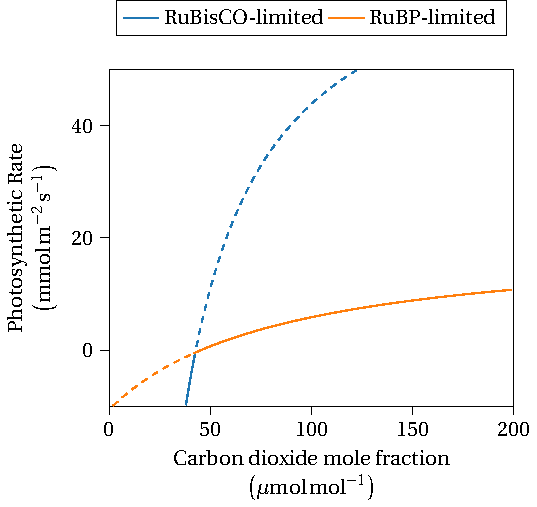
\includegraphics[scale=0.33]{figures/photosynthesis.pdf}
                \end{column}
                \begin{column}{0.3\textwidth}
                    \resizebox{\textwidth}{!}{
                        \begin{tikzpicture}[node distance=1cm]
                            \node (start) [startstop] {Start};
                
                            \node (in1) [init, below=of start] {$x_i = x_a$};
                
                            \node (pro1) [process, below=of in1] {$r_c = f_{r_c}(T_a,h_a,T_s,T_r,P)$};
                            \node (pro2) [process, below=of pro1] {$A = f_A(I, x_i, T_s)$};
                            \node (pro3) [process, below=of pro2] {$x_i^{\mathrm{new}} = x_a - A \cdot r_c$};
                
                            \node (dec1) [decision, below=of pro3] {$\vert x_i^{\mathrm{new}} - x_i \vert < \epsilon$};
                
                            \node (pro4) [process, left=of dec1] {$x_i = x_i^{\mathrm{new}}$};
                
                            \node (stop) [startstop, below=of dec1] {Stop};
                
                            \draw [arrow] (start) -- (in1);
                            \draw [arrow] (in1) -- (pro1);
                            \draw [arrow] (pro1) -- (pro2);
                            \draw [arrow] (pro2) -- (pro3);
                            \draw [arrow] (pro3) -- (dec1);
                            \draw [arrow] (dec1) -- node[midway, above] {no} (pro4);
                            \draw [arrow] (pro4) |- (pro2);
                            \draw [arrow] (dec1) -- node[midway, left] {yes} (stop);
                        \end{tikzpicture}
                    }
                \end{column}
            \end{columns}
        \end{column}
    \end{columns}

\end{frame}

\begin{frame}
    \frametitle{Neural Network I}

    \begin{columns}
        \begin{column}{0.6\textwidth}
            \only<1>{
                \begin{figure}
                    \centering
                    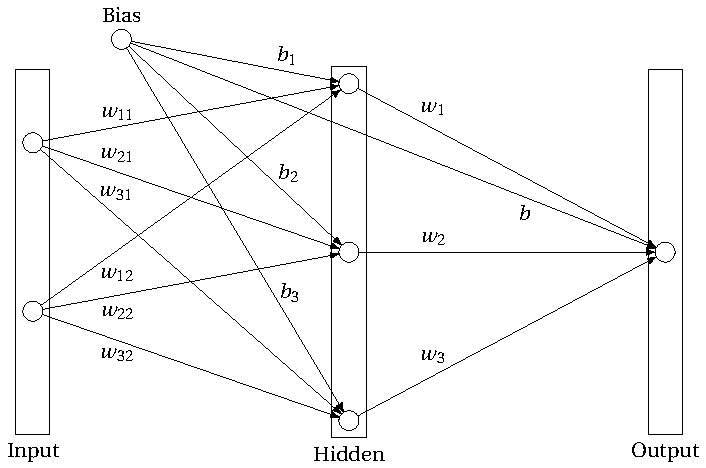
\includegraphics[scale=0.5]{figures/nn1.pdf}
                    \caption{Example three-layer neural network.}
                \end{figure}
            }
            \only<2>{
                \begin{figure}
                    \centering
                    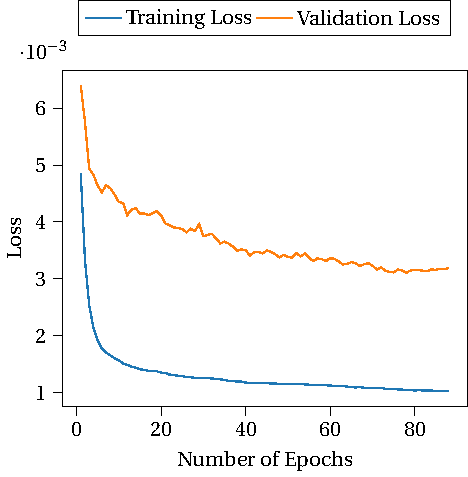
\includegraphics[scale=0.5]{figures/nn2.pdf}
                    \caption{Training and validation losses.}
                \end{figure}
            }
        \end{column}
        \begin{column}{0.4\textwidth}
            \begin{itemize}
                \item test 1
                \item test 2
            \end{itemize}
        \end{column}
    \end{columns}
\end{frame}

\begin{frame}
    \frametitle{Neural Network II}
    \begin{figure}
        \centering
        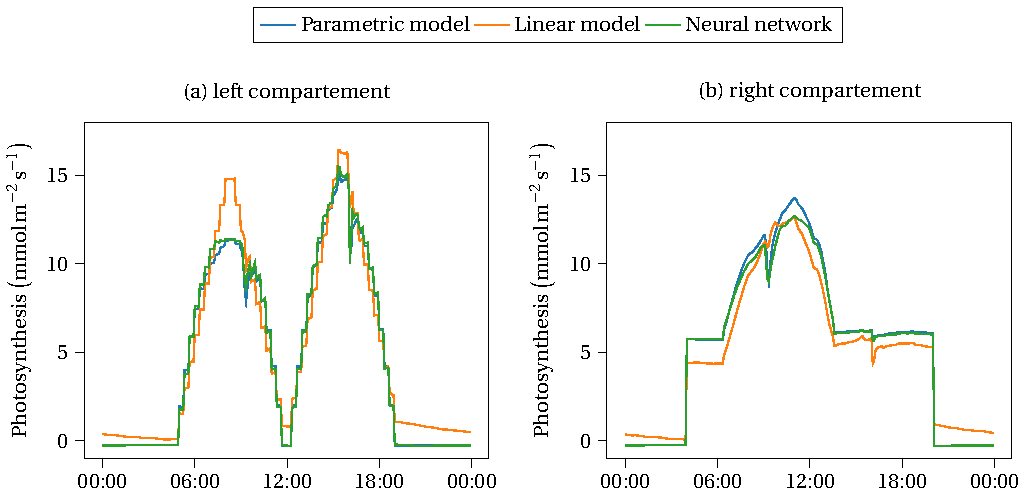
\includegraphics[scale=0.5]{figures/nn3.pdf}
        \caption{Photosynthetic rates for the (a) left and (b) right compartement.}
    \end{figure}
\end{frame}